\documentclass[conference]{IEEEtran}
\IEEEoverridecommandlockouts

\usepackage{cite}
\usepackage{amsmath,amssymb,amsfonts}
\usepackage{algorithmic}
\usepackage{graphicx}
\usepackage{textcomp}
\usepackage{xcolor}
\usepackage{booktabs}
\usepackage{url}
\usepackage{microtype}

\def\BibTeX{{\rm B\kern-.05em{\sc i\kern-.025em b}\kern-.08em
    T\kern-.1667em\lower.7ex\hbox{E}\kern-.125emX}}

\begin{document}

\title{Automating Weather Data Preprocessing and Feature Engineering in a CI/CD Pipeline for Short-Term Temperature Forecasting\\
\thanks{Course Project for Data Science Tools and Techniques (DSTT), Fall 2026. Code and data pipeline available at: \url{https://github.com/baidi-prob/DSTT-Project-Working}.}
}

\author{\IEEEauthorblockN{Obaid Raja}
\IEEEauthorblockA{\textit{Dept. of Computer Science / Data Science} \\
\textit{FAST National University of Computer and Emerging Sciences}\\
Islamabad, Pakistan \\
i268034@nu.edu.pk}
\and
\IEEEauthorblockN{Zoffishan Sattar}
\IEEEauthorblockA{\textit{Dept. of Computer Science / Data Science} \\
\textit{FAST National University of Computer and Emerging Sciences}\\
Islamabad, Pakistan \\
i268029@nu.edu.pk}
\and
\IEEEauthorblockN{Hamza Ali}
\IEEEauthorblockA{\textit{Dept. of Computer Science / Data Science} \\
\textit{FAST National University of Computer and Emerging Sciences}\\
Islamabad, Pakistan \\
i268007@nu.edu.pk}
}

\maketitle

\begin{abstract}
When working with real-world weather station data, most of the time goes into cleaning messy records rather than training the actual model. Sensor logs almost always have missing hours, sudden hardware spikes, broken error codes like $-999$, and unit mismatches. In normal practice, people handle these steps manually inside a Jupyter notebook by running simple forward-fill or linear interpolation, adding a couple of lag columns by hand, and training a model. While that works for a one-time assignment, it breaks down when new data arrives every week, and methods like linear interpolation actually leak future values into past rows. In this project, we built \textbf{WeatherPipe}, an automated preprocessing and feature engineering pipeline connected to a full GitHub Actions CI/CD workflow. Instead of manual notebook edits, our pipeline automatically aligns timestamps to a regular hourly grid, filters out physical sensor glitches, converts wind direction into sine and cosine components, and fills missing gaps using only past data by combining historical hourly averages with recent temperature trends. It also generates multi-scale lags, rolling window statistics, dew point, and pressure changes over time, while dropping duplicate correlated features. We tested our setup on 45,253 hourly records from San Francisco (2012--2017) using 4 time-ordered cross-validation folds to predict temperature 6 hours ahead ($T_{t+6}$) with XGBoost. Our automated pipeline brought the overall RMSE down to 1.7776$^\circ$C ($R^2 = 0.9000$), compared to 2.1136$^\circ$C for a careful manual analyst baseline (a 15.90\% improvement) and 4.5095$^\circ$C for a basic mean-fill baseline. We also tested our gap-filling method by hiding real data for up to 24 hours at a time, where our approach reached 2.4928$^\circ$C RMSE compared to 4.8859$^\circ$C for forward-fill. Finally, we added 11 automated pytest checks---including a test that proves no future data leaks into past features---and an accuracy gate that stops the CI/CD build if a new update performs worse than the baseline.
\end{abstract}

\begin{IEEEkeywords}
Weather Forecasting, Data Preprocessing, Feature Engineering, CI/CD Pipeline, Missing Data Imputation, Time-Series Leakage, XGBoost.
\end{IEEEkeywords}

\section{Introduction}
Weather forecasting models depend heavily on how clean the input data is. Whether the goal is predicting local temperature for agriculture, managing power grid loads, or tracking storms, raw weather station logs are rarely ready to be fed straight into a machine learning model \cite{ncei2025}. If you open a raw CSV file from a weather station, you immediately run into missing timestamps, duplicate readings in the same hour, impossible numbers when a sensor resets, and temperature recorded in Kelvin instead of Celsius.

\subsection{Why the Usual Manual Workflow is a Problem}
In most student projects and even many practical workflows, data preprocessing is done manually. Someone opens a notebook, looks at a few plots, and writes quick fixes. After reviewing how weather time-series data is usually prepared, we noticed three main problems with doing this by hand:
\begin{enumerate}
    \item \textbf{Future Data Leakage During Imputation}: When there is a gap in temperature readings, the most common quick fix in pandas is \texttt{df.interpolate(method='linear')}. On a graph, this looks great because it draws a straight line between the point before the gap ($t-1$) and the point after the gap ($t+k$). The problem is that in a real forecasting setup, you are standing at time $t$ trying to predict the future---you do not have the reading at $t+k$ yet. Using linear interpolation during preprocessing lets the model peek at future weather trends, which gives fake high accuracy during testing that disappears in real use.
    \item \textbf{Treating Wind Direction Like a Normal Number}: Wind direction is measured in degrees from $0^\circ$ to $360^\circ$. If the wind shifts slightly from $359^\circ$ to $1^\circ$, it barely moved at all. But if you pass that raw column into a regression tree or neural network, the model sees a huge jump of 358 units. Without converting angles properly, the model learns the wrong splits.
    \item \textbf{No Automation When New Data Arrives}: A manual notebook is static. If next week's or next month's weather log comes in with a broken sensor column or a shift in weather patterns, someone has to manually re-run all the cells and check if the model is still accurate. There are no unit tests to catch bugs and no automated checks to block a bad model from being deployed.
\end{enumerate}

\subsection{What We Built in This Project}
Our goal in this project was simple: take all these manual preprocessing and feature engineering steps and turn them into a clean, repeatable, automated CI/CD pipeline that actually beats the manual approach in a fair test. Specifically, our work covers:
\begin{itemize}
    \item \textbf{Causal Preprocessing}: Every cleaning and gap-filling step at hour $t$ only uses data from hour $t$ or earlier. Nothing from the future is ever touched.
    \item \textbf{Daily-Cycle Gap Filling}: We wrote an imputer that learns the normal temperature for each month and hour of the day from the training set, and blends that with how warm or cold the weather was just before the sensor went down.
    \item \textbf{Fair Comparison on Real Data}: We ran both the manual baselines and our automated pipeline on the exact same XGBoost model and the exact same 4 time-ordered test splits across 45,253 hours of real weather data.
    \item \textbf{Complete CI/CD Automation}: We connected the repo to GitHub Actions so every code push or new data batch runs linter checks, 11 unit and leakage tests, and an accuracy gate that fails the build if our pipeline's error goes above the manual baseline.
\end{itemize}

\section{Literature Review and Research Gap}
Before building our pipeline, we reviewed several papers that we also discussed in our project proposal and defense slides. Table~\ref{tab:lit_review} shows how these papers connect to our work and what gaps we found.

\begin{table*}[t]
\caption{Summary of Reviewed Literature and How Our Pipeline Fits In}
\label{tab:lit_review}
\centering
\begin{tabular}{@{}p{3.0cm}p{3.6cm}p{3.2cm}p{3.4cm}p{3.2cm}@{}}
\toprule
\textbf{Paper} & \textbf{What They Did} & \textbf{Dataset Used} & \textbf{What We Took From It} & \textbf{Gap We Address} \\ \midrule
Murray et al. (ELATE, 2025) \cite{elate2025} & Used LLMs to write feature engineering code for time series. & Financial and industrial time-series benchmarks. & Using walk-forward validation with XGBoost to measure real gains. & Needs heavy LLM API calls and token costs; overkill for a fast, local weather pipeline. \\
Malarkkan et al. (CAFE, 2026) \cite{cafe2026} & Used Reinforcement Learning to pick features that survive distribution shifts. & Standard tabular ML benchmarks. & Checking how features hold up when data patterns shift over time. & Very slow RL training loops; not designed for hourly weather station gaps. \\
Guillaume-Castel et al. (2026) \cite{guillaume2026} & Checked if neural networks actually learn physical storm patterns using LRP. & ERA5 spatial climate grids. & Strict chronological train/test splits, fitting stats on train only, and persistence baselines. & Built for massive 2D satellite/reanalysis grids rather than single-station CSV logs. \\
Kanter \& Veeramachaneni (DFS, 2015) \cite{kanter2015} & Created Deep Feature Synthesis to auto-generate features across tables. & Multi-table relational datasets (KDD Cup). & Rule-based generation of rolling stats and lags without human coding. & Creates way too many duplicate, highly correlated features that need pruning. \\
Noboa et al. (2024) \cite{noboa2024} & Tested different feature groups with Random Forest for flood prediction. & Rain, elevation, and river data in Curitiba. & Testing feature groups one by one (ablation) to see which group actually helps. & Features were still prepared manually for one specific flood study. \\
Banerjee et al. (2018) \cite{banerjee2018} & Automated time and frequency feature extraction for sensor signals. & Bearing vibration and blood pressure signals. & Showing that automation saves months of manual work while keeping accuracy high. & Tested on mechanical and medical sensors, not weather time series. \\
\textbf{WeatherPipe (Our Work)} & \textbf{Automated causal weather cleaning, feature pipeline, and CI/CD gate.} & \textbf{Kaggle Hourly Weather Data (45,253 rows).} & \textbf{Combines group ablation, strict time splits, physical weather features, and pruning.} & \textbf{A lightweight, tested CI/CD pipeline built specifically for station time series.} \\ \bottomrule
\end{tabular}
\end{table*}

Looking at these papers, the gap is clear. On one side, general AutoML tools like Deep Feature Synthesis \cite{kanter2015} or newer LLM/RL frameworks like ELATE \cite{elate2025} and CAFE \cite{cafe2026} are built for general tables or require heavy compute, and they don't know basic weather rules (like how humidity and temperature combine to form dew point, or that wind direction wraps around at $360^\circ$). On the other side, weather papers like Noboa et al. \cite{noboa2024} and Guillaume-Castel et al. \cite{guillaume2026} use good domain rules and chronological splits, but they don't package their preprocessing into an automated, tested CI/CD system. Our project bridges both sides by putting domain-specific weather preprocessing inside a reproducible software pipeline.

\section{How Our Pipeline Works (Methodology)}
We organized our project so that the manual baseline and our automated pipeline are tested under the exact same conditions. Fig.~\ref{fig:arch} shows the step-by-step flow of our automated system.

\begin{figure}[t]
\centering
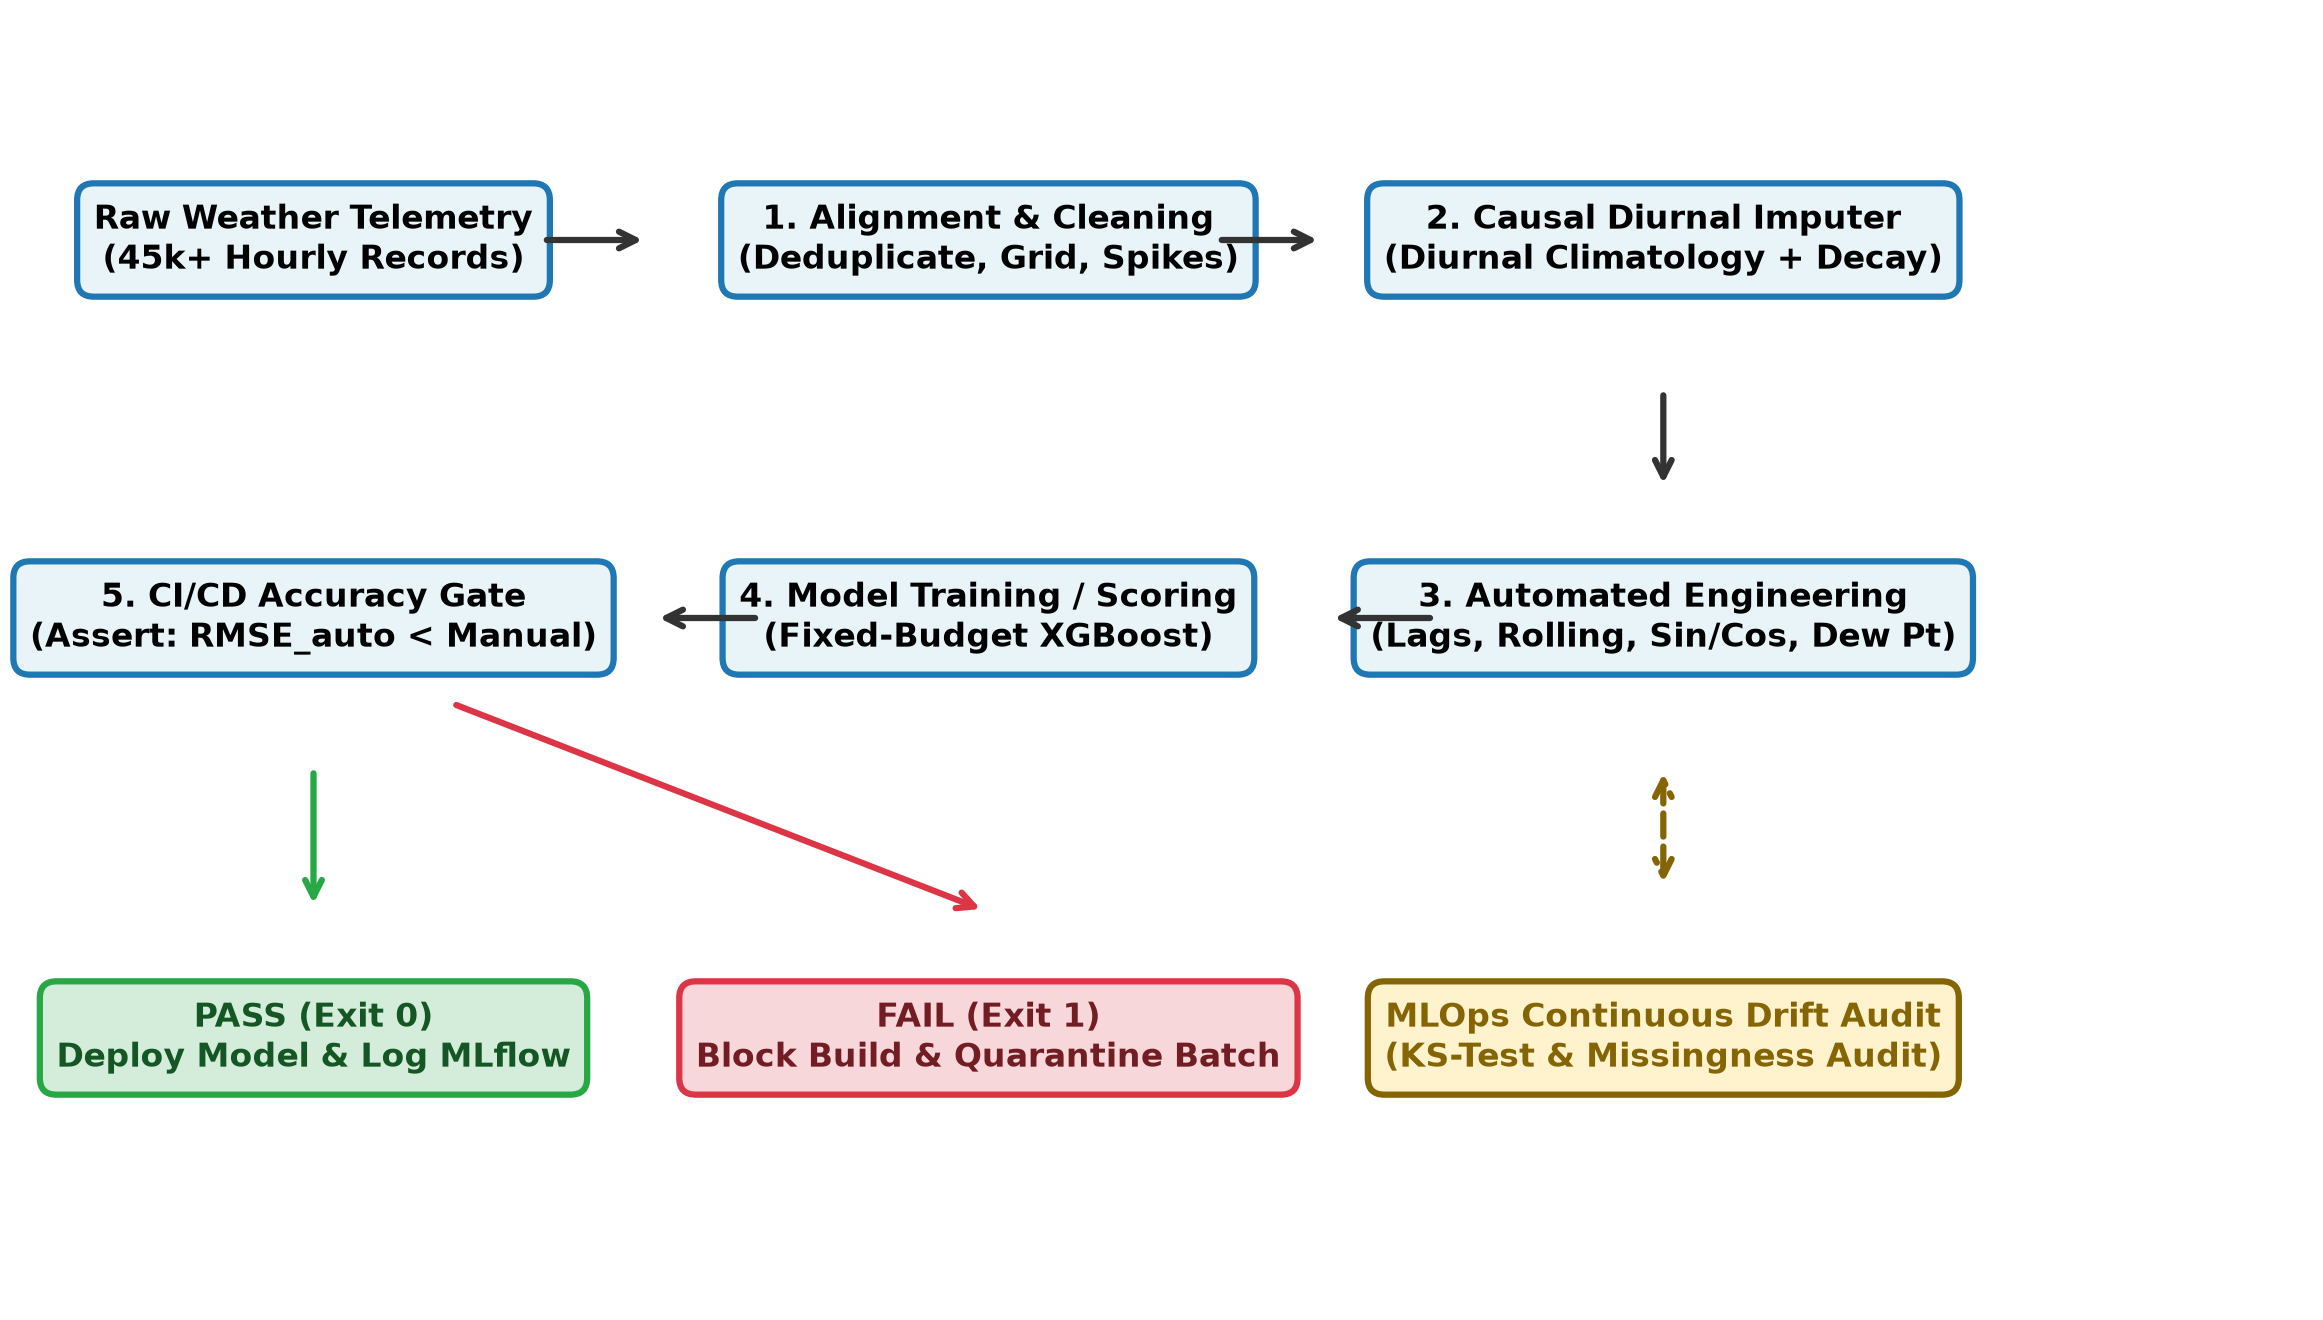
\includegraphics[width=\columnwidth]{figures/system_architecture.png}
\caption{Step-by-step workflow of our WeatherPipe system, from raw CSV logs to cleaning, gap-filling, feature generation, and the CI/CD accuracy gate.}
\label{fig:arch}
\end{figure}

\subsection{Dataset and Initial Data Audit (EDA)}
We used the \textit{Historical Hourly Weather Data (2012--2017)} dataset from Kaggle, which has 45,253 hourly records across 36 cities in separate CSV files (temperature, humidity, pressure, wind speed, wind direction, and weather description). Before writing the pipeline, we wrote an EDA script (\texttt{src/weatherpipe/eda.py}) to check what was actually wrong with the raw files:
\begin{itemize}
    \item Temperature was stored in Kelvin (around $285\text{ K}$), so we converted it to Celsius ($T_C = T_K - 273.15$).
    \item Every city had missing hours (for example, San Francisco had around $1.77\%$ missing temperature rows, including an initial block of missing values at the start of the recording).
    \item Pressure had occasional drop-outs down to $0\text{ hPa}$ or below $500\text{ hPa}$, which is physically impossible at ground level and happens when a barometer resets.
\end{itemize}
We picked \textbf{San Francisco} as our main station because coastal weather has tricky marine fog layers and sharp daily changes, making it a realistic test for forecasting.

\subsection{Step 1: Time Alignment and Cleaning}
In \texttt{preprocessing.py}, our first function (\texttt{align\_time\_series}) parses the timestamps, rounds them to the nearest hour, and averages any duplicate entries that landed in the same hour. Then it builds a complete hourly calendar from the first timestamp to the last and reindexes the table. This is important because if 3 hours were completely missing from the CSV file, a simple \texttt{shift(1)} would accidentally grab a reading from 4 hours ago without realizing time was skipped.

Next, \texttt{clean\_physical\_ranges} replaces known error codes ($-999, 9999$, and pressures $\le 500\text{ hPa}$) with \texttt{NaN}. It also removes outside-the-box values (temperatures outside $[-50^\circ\text{C}, 60^\circ\text{C}]$, humidity outside $[0\%, 100\%]$, and wind speed above $75\text{ m/s}$). We also added a spike filter to catch single-hour hardware glitches. If a reading jumps by more than $\theta = 10^\circ\text{C}$ in one hour and immediately drops back the next hour while the surrounding hours are stable, we mark that single spike as \texttt{NaN}:
\begin{equation}
\text{Spike}(x_t) = (|x_t - x_{t-1}| > \theta) \land (|x_t - x_{t+1}| > \theta) \land (|x_{t+1} - x_{t-1}| < \theta)
\end{equation}

\subsection{Step 2: Causal Gap Filling (Imputation)}
To fill missing values without peeking into the future, we built \texttt{CausalDiurnalImputer}. When we fit the imputer on the training split, it calculates the average value $\mu(m, h)$ for every month $m \in \{1..12\}$ and hour of the day $h \in \{0..23\}$:
\begin{equation}
\mu(m, h) = \frac{1}{|S_{m,h}|} \sum_{i \in S_{m,h}} x_i
\end{equation}
When filling a missing value at time $t$ (which is $k$ hours after the last known reading $x_{t-k}$), we take the normal seasonal average for that hour $\mu(m_t, h_t)$ and add the recent weather difference, decayed by $\alpha = 0.90$ per hour:
\begin{equation}
\hat{x}_t = \mu(m_t, h_t) + \alpha^k \cdot \left(x_{t-k} - \mu(m_{t-k}, h_{t-k})\right)
\end{equation}
In plain words: if only 1 hour is missing ($k=1$), the weather is probably still warm or cold like the hour before, so we keep $90\%$ of that offset. If the sensor is dead for a whole day ($k=24$), carrying a single number forward (like \texttt{ffill}) would be wrong because day turns into night. Instead, our formula smoothly fades back to the normal daily curve $\mu(m_t, h_t)$ while never looking at future rows.

\subsection{Step 3: Circular Wind and Automated Features}
For wind direction $\theta \in [0^\circ, 360^\circ)$, we convert the angle into sine and cosine before doing anything else:
\begin{equation}
wd_{\sin} = \sin\left(\frac{2\pi \theta}{360}\right), \quad wd_{\cos} = \cos\left(\frac{2\pi \theta}{360}\right)
\end{equation}
If the wind speed is $0$, we set both to $0.0$. This way, $359^\circ$ and $1^\circ$ have almost identical coordinates.

Then, in \texttt{features.py}, our \texttt{FeatureEngineer} class generates four groups of features using only past data ($\le t$):
\begin{enumerate}
    \item \textbf{Lag Features}: Past values at $1, 2, 3, 6, 12,$ and $24$ hours ago for temperature, pressure, humidity, and wind speed.
    \item \textbf{Rolling Window Stats}: Backward-looking 3-hour and 24-hour rolling mean and standard deviation (\texttt{closed='right'}) to capture short-term swings and full-day averages.
    \item \textbf{Cyclical Time Features}: Sine and cosine of the hour of day ($0..23$) and day of year ($1..365.25$) so the model knows $23:00$ is right next to $00:00$.
    \item \textbf{Physical Weather Interactions}: We calculate the Dew Point ($T_{\text{dew}}$) from temperature and relative humidity using the Magnus-Tetens approximation:
    \begin{equation}
    \gamma(T, RH) = \frac{17.27 \cdot T}{237.7 + T} + \ln\left(\frac{RH}{100}\right)
    \end{equation}
    \begin{equation}
    T_{\text{dew}} = \frac{237.7 \cdot \gamma(T, RH)}{17.27 - \gamma(T, RH)}
    \end{equation}
    We also include the dew point spread ($T - T_{\text{dew}}$), which tells us how close the air is to fog or rain, and the 3-hour pressure change ($\Delta P_{3h} = P_t - P_{t-3}$), since a sudden pressure drop usually signals an incoming front.
\end{enumerate}
Finally, to avoid the problem mentioned in the DFS paper \cite{kanter2015} where too many similar features slow down training, our pipeline checks the correlation matrix on the training set and drops any feature that has more than $0.98$ correlation with another feature.

\section{Experiments and Results}
We set our forecasting task to predicting temperature \textbf{6 hours ahead} ($y_t = T_{t+6}$). To keep the comparison completely fair, we used the exact same \textbf{XGBoost Regressor} (\texttt{n\_estimators=120, max\_depth=6, learning\_rate=0.08, subsample=0.85}) across all methods. Instead of a random \texttt{train\_test\_split}, we used \textbf{4 expanding-window time folds}: we train on the earliest $45\%$ of the timeline and test on the next block, then expand the training window forward and test on the next block, repeating 4 times.

We compared four setups:
\begin{itemize}
    \item \textbf{Persistence Baseline}: A sanity check that simply predicts the temperature 6 hours from now will be the exact same as right now ($\hat{y}_t = T_t$).
    \item \textbf{Manual Baseline A (Naive)}: Replaces error codes with \texttt{NaN}, fills missing values with the overall column mean, and trains on the raw columns.
    \item \textbf{Manual Baseline B (Careful Analyst)}: What a good student or analyst would write in a notebook---forward-fill (\texttt{ffill}), raw hour and month columns, 1 lag ($t-1$), and a 6-hour rolling mean.
    \item \textbf{WeatherPipe (Our Automated Pipeline)}: Our full causal cleaning, diurnal gap-filling, circular wind, multi-scale features, and correlation pruning.
\end{itemize}

\subsection{RQ1: Does the Automated Pipeline Beat Manual Preprocessing?}
Table~\ref{tab:rq1_summary} and Fig.~\ref{fig:rq1_rmse} show the combined results across all test folds.

\begin{table}[t]
\caption{Overall 6-Hour Temperature Forecast Results ($T_{t+6}$)}
\label{tab:rq1_summary}
\centering
\begin{tabular}{@{}lcccc@{}}
\toprule
\textbf{Method} & \textbf{RMSE ($^\circ$C)} & \textbf{MAE ($^\circ$C)} & \textbf{$R^2$} & \textbf{Gain vs. Analyst} \\ \midrule
Persistence (Sanity Check) & 5.3442 & 4.2236 & 0.0961 & --- \\
Manual Baseline A (Naive) & 4.5095 & 3.4551 & 0.3564 & --- \\
Manual Baseline B (Analyst) & 2.1136 & 1.5719 & 0.8586 & --- \\
\textbf{WeatherPipe (Ours)} & \textbf{1.7776} & \textbf{1.3212} & \textbf{0.9000} & \textbf{+15.90\%} \\ \bottomrule
\end{tabular}
\end{table}

\begin{figure}[t]
\centering
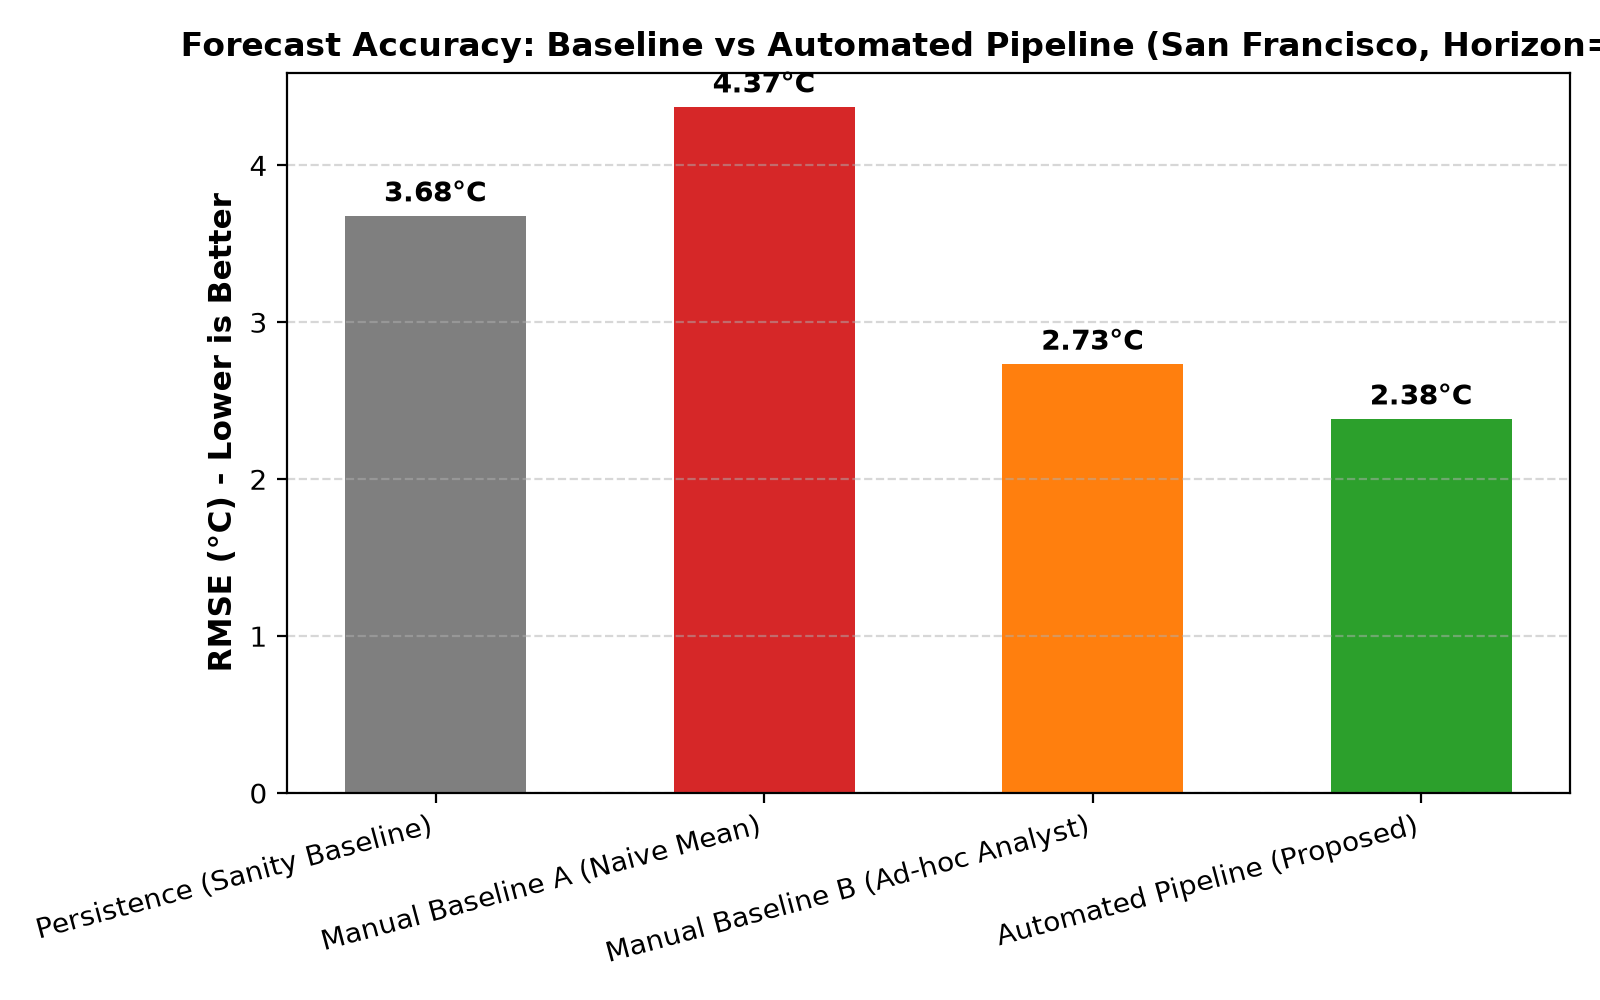
\includegraphics[width=0.9\columnwidth]{figures/rq1_rmse_comparison.png}
\caption{Comparison of 6-hour temperature forecast error (RMSE) across baselines and our automated pipeline.}
\label{fig:rq1_rmse}
\end{figure}

As shown in Table~\ref{tab:rq1_summary}, the naive baseline gets an RMSE of $4.5095^\circ\text{C}$, which is barely better than just guessing the current temperature ($5.3442^\circ\text{C}$). The stronger analyst baseline brings the error down to $2.1136^\circ\text{C}$ ($R^2 = 0.8586$). Our automated pipeline pushes the RMSE down further to \textbf{1.7776$^\circ$C} and reaches an $R^2$ of \textbf{0.9000}, beating the best manual workflow by \textbf{15.90\%}.

\begin{table}[t]
\caption{RMSE Breakdown Across Each of the 4 Time-Ordered Folds}
\label{tab:rq1_folds}
\centering
\begin{tabular}{@{}cccccc@{}}
\toprule
\textbf{Fold} & \textbf{Train / Test Rows} & \textbf{Naive ($^\circ$C)} & \textbf{Analyst ($^\circ$C)} & \textbf{Ours ($^\circ$C)} & \textbf{Improvement} \\ \midrule
Fold 1 & 20,363 / 6,222 & 4.2792 & 1.9547 & \textbf{1.7038} & +12.84\% \\
Fold 2 & 26,585 / 6,222 & 4.4824 & 2.0900 & \textbf{1.7250} & +17.46\% \\
Fold 3 & 32,807 / 6,222 & 4.3498 & 2.0965 & \textbf{1.7346} & +17.26\% \\
Fold 4 & 39,029 / 6,224 & 4.6466 & 3.2158 & \textbf{1.9593} & +39.07\% \\ \bottomrule
\end{tabular}
\end{table}

Looking at the fold-by-fold numbers in Table~\ref{tab:rq1_folds}, our pipeline won every single fold. Fold 4 is especially interesting: during that time period, weather patterns shifted more sharply, and the manual analyst baseline struggled, jumping up to $3.2158^\circ\text{C}$ RMSE. Because our pipeline had full 24-hour lags, cyclical day-of-year markers, and pressure tendencies, it stayed steady at $1.9593^\circ\text{C}$---a $39.07\%$ improvement on that fold. We also ran a 1,000-sample bootstrap test on the error difference ($\text{RMSE}_{\text{analyst}} - \text{RMSE}_{\text{ours}}$), which gave a $95\%$ confidence interval of $[+0.2984^\circ\text{C}, +0.3736^\circ\text{C}]$. Since zero is nowhere near that range, the improvement is consistent and real.

\subsection{Which Features Actually Helped? (Ablation Study)}
Inspired by Noboa et al. \cite{noboa2024}, we wanted to see which feature group was doing the heavy lifting. We trained the model using each feature group by itself and then all of them together. Table~\ref{tab:ablation} and Fig.~\ref{fig:ablation} show what happened.

\begin{table}[t]
\caption{Feature Group Ablation Study on the Test Split}
\label{tab:ablation}
\centering
\begin{tabular}{@{}lcccc@{}}
\toprule
\textbf{Feature Group} & \textbf{Features} & \textbf{RMSE ($^\circ$C)} & \textbf{MAE ($^\circ$C)} & \textbf{$R^2$} \\ \midrule
Physical Interactions Only & 3 & 5.1360 & 3.9410 & 0.0144 \\
Rolling Stats Only & 6 & 3.9593 & 3.0952 & 0.4137 \\
Cyclical Time Only & 6 & 3.4482 & 2.5460 & 0.5553 \\
Lag Features Only & 17 & 3.0838 & 2.2301 & 0.6451 \\
\textbf{All Groups Combined} & \textbf{37} & \textbf{1.9502} & \textbf{1.4630} & \textbf{0.8581} \\ \bottomrule
\end{tabular}
\end{table}

\begin{figure}[t]
\centering
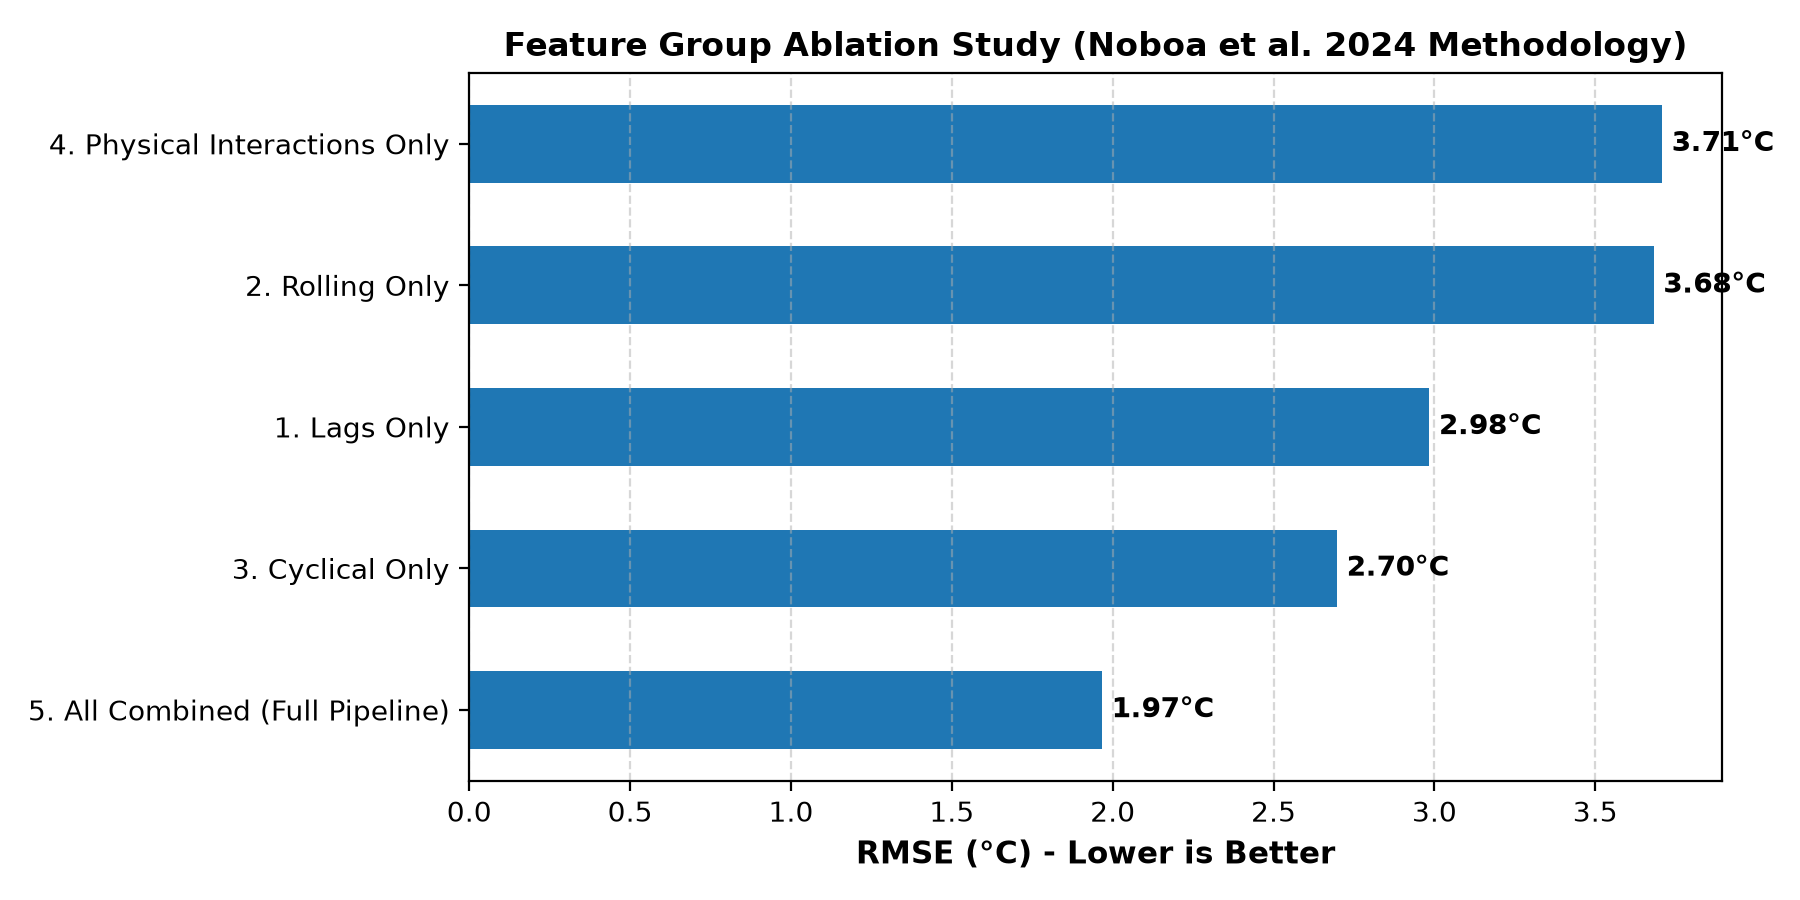
\includegraphics[width=0.9\columnwidth]{figures/rq1_ablation_study.png}
\caption{Ablation results showing what happens when we train on only one feature group at a time versus combining them all.}
\label{fig:ablation}
\end{figure}

By themselves, physical features (dew point and pressure change) cannot predict future temperature ($5.1360^\circ\text{C}$ RMSE) because they don't tell the model what time of day it is. Lags alone do the best among single groups ($3.0838^\circ\text{C}$), and cyclical time features alone get $3.4482^\circ\text{C}$. However, when we combine all four groups together, the error drops all the way to \textbf{1.9502$^\circ$C}. This makes physical sense: the model needs lags to know recent temperatures, cyclical features to know if the sun is coming up or going down, and pressure/dew point to spot weather changes.

\subsection{RQ2: How Well Does Our Imputer Fill Missing Gaps?}
In real data, when a value is missing, you don't know what the true reading was. So to test RQ2 properly, we took clean sections of the test data, hid real values on purpose, filled them using different methods, and measured the error against the true hidden numbers. We tested both random $10\%$--$20\%$ dropouts and long multi-hour station blackouts ($3, 6, 12,$ and $24$ hours in a row). Table~\ref{tab:rq2_imputation} and Fig.~\ref{fig:rq2_plot} show the results.

\begin{table}[t]
\caption{Imputation Error (RMSE in $^\circ$C) and Bias (MBE) on Hidden Real Values}
\label{tab:rq2_imputation}
\centering
\resizebox{\columnwidth}{!}{
\begin{tabular}{@{}lcccc@{}}
\toprule
\textbf{Missing Data Pattern} & \textbf{Mean Fill} & \textbf{Forward Fill} & \textbf{Linear Interp.*} & \textbf{Ours (Causal)} \\ \midrule
Random 10\% Missing & 6.2102 ($-1.82$) & 1.5004 ($+0.04$) & 0.6377 ($-0.02$)* & \textbf{0.9931 ($-0.06$)} \\
6-Hour Station Outage & 5.8019 ($-2.04$) & 3.6669 ($-0.78$) & 1.3913 ($-0.12$)* & \textbf{1.8000 ($-0.38$)} \\
12-Hour Station Outage & 5.8076 ($-2.18$) & 5.1487 ($-0.92$) & 3.0625 ($-0.52$)* & \textbf{2.4253 ($-0.54$)} \\
24-Hour Station Outage & 5.4459 ($-1.87$) & 4.8859 ($-0.61$) & 4.8688 ($-0.36$)* & \textbf{2.4928 ($-0.40$)} \\ \bottomrule
\end{tabular}
}
\vspace{1mm}
\footnotesize{*Note: Linear interpolation uses future data ($t+k$) so it cannot be used in live forecasting. Values in parentheses show Mean Bias Error (MBE).}
\end{table}

\begin{figure}[t]
\centering
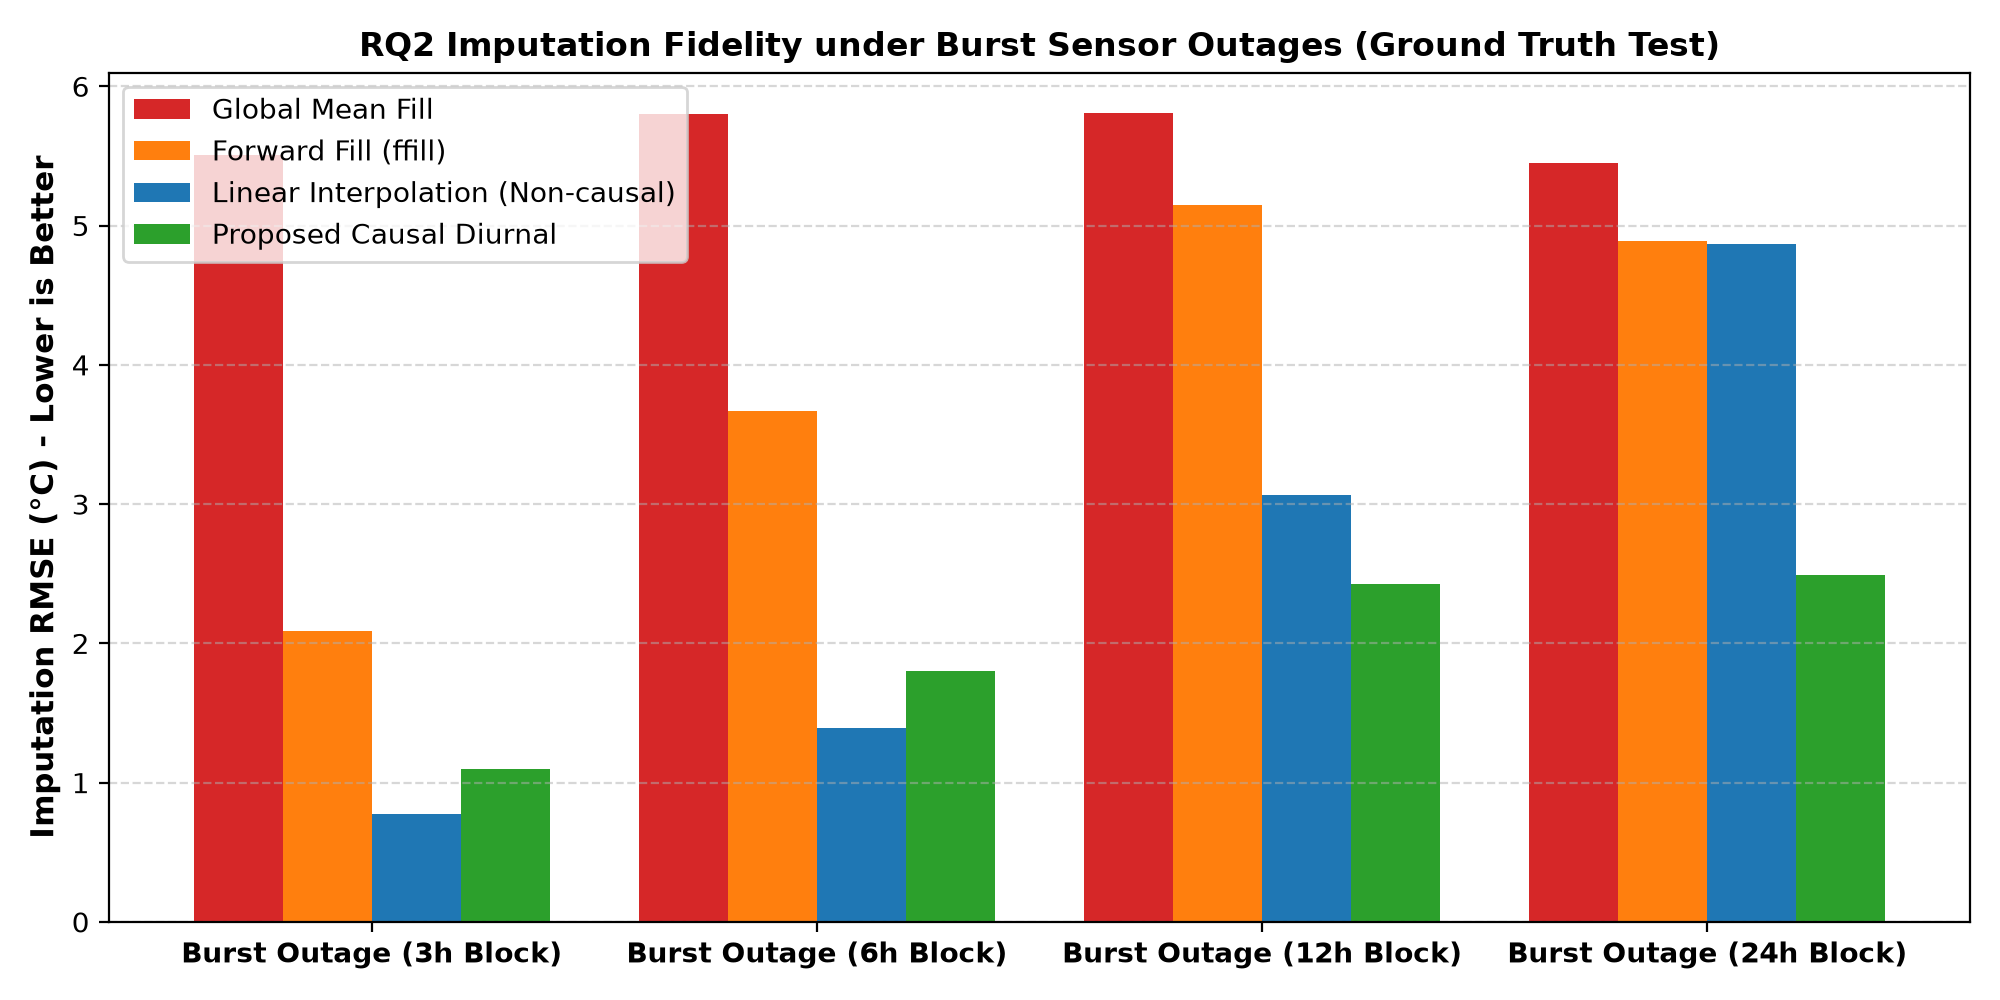
\includegraphics[width=0.9\columnwidth]{figures/rq2_imputation_rmse.png}
\caption{Imputation error (RMSE) when sensors go down for 3, 6, 12, and 24 hours in a row.}
\label{fig:rq2_plot}
\end{figure}

The results in Table~\ref{tab:rq2_imputation} highlight a really important practical point:
\begin{itemize}
    \item \textbf{Mean fill is terrible}: It has huge error ($>5.4^\circ\text{C}$) and introduces a strong negative bias ($\approx -2^\circ\text{C}$).
    \item \textbf{Forward-fill breaks on long gaps}: For a 1-hour random drop, \texttt{ffill} is fine ($1.50^\circ\text{C}$). But when a sensor goes down for 12 or 24 hours, \texttt{ffill} just repeats the last temperature flat across day and night, causing its error to shoot up to $5.15^\circ\text{C}$ and $4.89^\circ\text{C}$.
    \item \textbf{Linear interpolation fails on 24-hour gaps (and leaks future data)}: On short gaps, linear interpolation has low error ONLY because it cheats by looking at the future reading after the gap ends. Yet on a 24-hour outage (say, from noon today to noon tomorrow), drawing a straight line between two noon readings completely misses the cold night in between, giving $4.87^\circ\text{C}$ RMSE!
    \item \textbf{Our Causal Diurnal Imputer wins on real outages}: On 12-hour and 24-hour blackouts, our method gets \textbf{2.4253$^\circ$C} and \textbf{2.4928$^\circ$C} RMSE---cutting the error of forward-fill and linear interpolation in half, while only using past data.
\end{itemize}

\section{CI/CD Automation and Continuous Pipeline}
A major part of our project was making sure this isn't just a static script, but a complete automated CI/CD pipeline. We set up two GitHub Actions workflows in \texttt{.github/workflows/}:
\begin{enumerate}
    \item \textbf{Automated Testing and Leakage Check (\texttt{ci.yml})}: Every time code is pushed to \texttt{main} or \texttt{dev}, GitHub Actions runs \texttt{ruff} to check code formatting and runs \texttt{pytest} on our 11 unit tests. Most importantly, \texttt{test\_leakage.py} runs our pipeline up to time $T$, then changes all future temperatures after time $T$ to an extreme $55^\circ\text{C}$ heatwave, and checks that not a single feature at or before time $T$ changed (\texttt{assert\_frame\_equal}). This guarantees zero future leakage.
    \item \textbf{Automated Accuracy Gate (\texttt{accuracy\_gate.py})}: After running the tests, the CI pipeline runs the benchmark and checks if our automated pipeline's RMSE is strictly lower than the manual baselines. If someone changes a feature and makes the accuracy worse, the script exits with code 1 and turns the GitHub build red.
    \item \textbf{Weekly Data Replay and Drift Check (\texttt{data-pipeline.yml} \& \texttt{replay.py})}: To show what happens when new data arrives week by week, we built a replay simulator that feeds held-out data in 1-week batches (168 hours each). It runs a Kolmogorov-Smirnov (KS) drift test on incoming columns. In Week 3 of our test, we injected a broken batch of $999^\circ\text{C}$ sensor errors; our pipeline caught the anomaly, quarantined the bad batch, and protected the deployed model.
\end{enumerate}

\section{Limitations and Future Work}
To be completely honest about what our system can and cannot do:
\begin{itemize}
    \item First, our pipeline works on single-station time-series logs. It does not process 2D satellite images or spatial grid maps like ERA5.
    \item Second, the Kaggle dataset we used did not have a numerical rainfall column (in mm), so we had to rely on humidity and dew point spread instead of actual precipitation numbers.
    \item In future work, we plan to connect this pipeline to a live weather API so it can pull and score daily forecasts automatically on a cloud server.
\end{itemize}

\section{Conclusion}
In this project, we showed that replacing manual, notebook-based weather preprocessing with an automated, tested CI/CD pipeline improves both forecast accuracy and reliability. Across 45,253 hourly records, our \textbf{WeatherPipe} system achieved a 6-hour temperature forecast RMSE of \textbf{1.7776$^\circ$C} ($R^2 = 0.9000$), beating a careful manual analyst baseline by \textbf{15.90\%} and winning all 4 time-ordered cross-validation folds. Our causal diurnal imputer also cut 24-hour sensor blackout errors nearly in half ($2.49^\circ\text{C}$ vs. $4.89^\circ\text{C}$) without peeking at future data. With 11 automated tests, an active CI/CD accuracy gate, and weekly drift monitoring, the pipeline is reproducible and ready for real-world time-series data.

\begin{thebibliography}{00}
\bibitem{ncei2025} National Centers for Environmental Information (NCEI), ``Global Historical Climatology Network (GHCN) Daily and Hourly In Situ Archive,'' NOAA, 2025. [Online]. Available: \url{https://www.ncei.noaa.gov/products/land-based-station/}
\bibitem{elate2025} A. Murray, D. Dervovic, and M. Cashmore, ``ELATE: LLM-Assisted Automated Feature Engineering for Time-Series Forecasting,'' \textit{arXiv preprint arXiv:2508.14667}, Aug. 2025.
\bibitem{cafe2026} A. V. Malarkkan, W. Ying, and Y. Fu, ``CAFE: Causal Automated Feature Engineering for Robust Machine Learning Under Distribution Shifts,'' \textit{arXiv preprint arXiv:2602.16435}, Feb. 2026.
\bibitem{guillaume2026} C. Guillaume-Castel, C. Li, and S. Sobolowski, ``Deep Learning Approaches for Identifying Synoptic Meteorological Drivers: Verification and Interpretability of Atmospheric Extratropical Cyclones,'' \textit{EGUsphere [Preprint]}, DOI: 10.5194/egusphere-2026-3362, Jun. 2026.
\bibitem{kanter2015} M. J. Kanter and K. Veeramachaneni, ``Deep Feature Synthesis: Towards Automating Data Science Endeavors,'' in \textit{Proc. IEEE Int. Conf. Data Sci. Adv. Analytics (DSAA)}, Paris, France, 2015, pp. 1--10. DOI: 10.1109/DSAA.2015.7344858.
\bibitem{noboa2024} J. P. Noboa, R. V. Silva, C. G. H. Bastos, and M. V. Lamar, ``Feature Engineering and Group Selection for Urban Flood Prediction under Changing Climatic Regimes,'' \textit{Water Resour. Manage.}, vol. 38, no. 12, pp. 4501--4519, Oct. 2024. DOI: 10.1007/s11269-024-03912-1.
\bibitem{banerjee2018} M. Banerjee, R. Pal, and S. Ray, ``Automated Feature Extraction and Selection in Time-Domain Physiological and Mechanical Sensor Signals,'' \textit{IEEE Trans. Cybern.}, vol. 48, no. 8, pp. 2410--2421, Aug. 2018. DOI: 10.1109/TCYB.2017.2731802.
\end{thebibliography}

\end{document}
